\chapterimage{chapter_head_2.pdf} % Chapter heading image

\chapter{Introdução}
%%%%%%%%%%%%%%%%%%%%%%%%%%%%%%%%%%%%%%%%%%%%%%%%%%%%%%%%%%%%%%%%%%%%%%%%%%%%%%%%
%% SECTION
%%%%%%%%%%%%%%%%%%%%%%%%%%%%%%%%%%%%%%%%%%%%%%%%%%%%%%%%%%%%%%%%%%%%%%%%%%%%%%%%
\section{Historia da samba}\index{historia da samba}
O samba é uns dos gêneros musicais mais conhecidos no Brasil \cite[pp. 46-47]{diniz2008almanaque},
entre estes gêneros mais populares temos por exemplo o ``forró'' e o ``Sertanejo'';
sendo que o samba se distingue entre eles, como a principal expressão popular da música brasileira. 


%O gênero samba atual é uma mistura de muitos gêneros musicais de África, América e Europa.

No inicios do seculo XIX os viajantes portugueses designavam as danças africanas com a palavra ``batuque'',
e no Brasil existem registros desta palavra desde o século XVIII, sendo que
esta não se usava para referenciar uma dança em particular e sim aos festejos dos negros em geral.
Assim, a designação  ``batuque'' foi muito popular ate inícios do seculo XX onde a palavra ``samba''
 virou mais popular para descrever estes festejos, Ver Figura \ref{fig:sambacrono}. 
\cite[pp. 85]{sandroni2001feitico} \cite[pp. 47]{diniz2008almanaque}.
\begin{figure}[h]
  \centering
    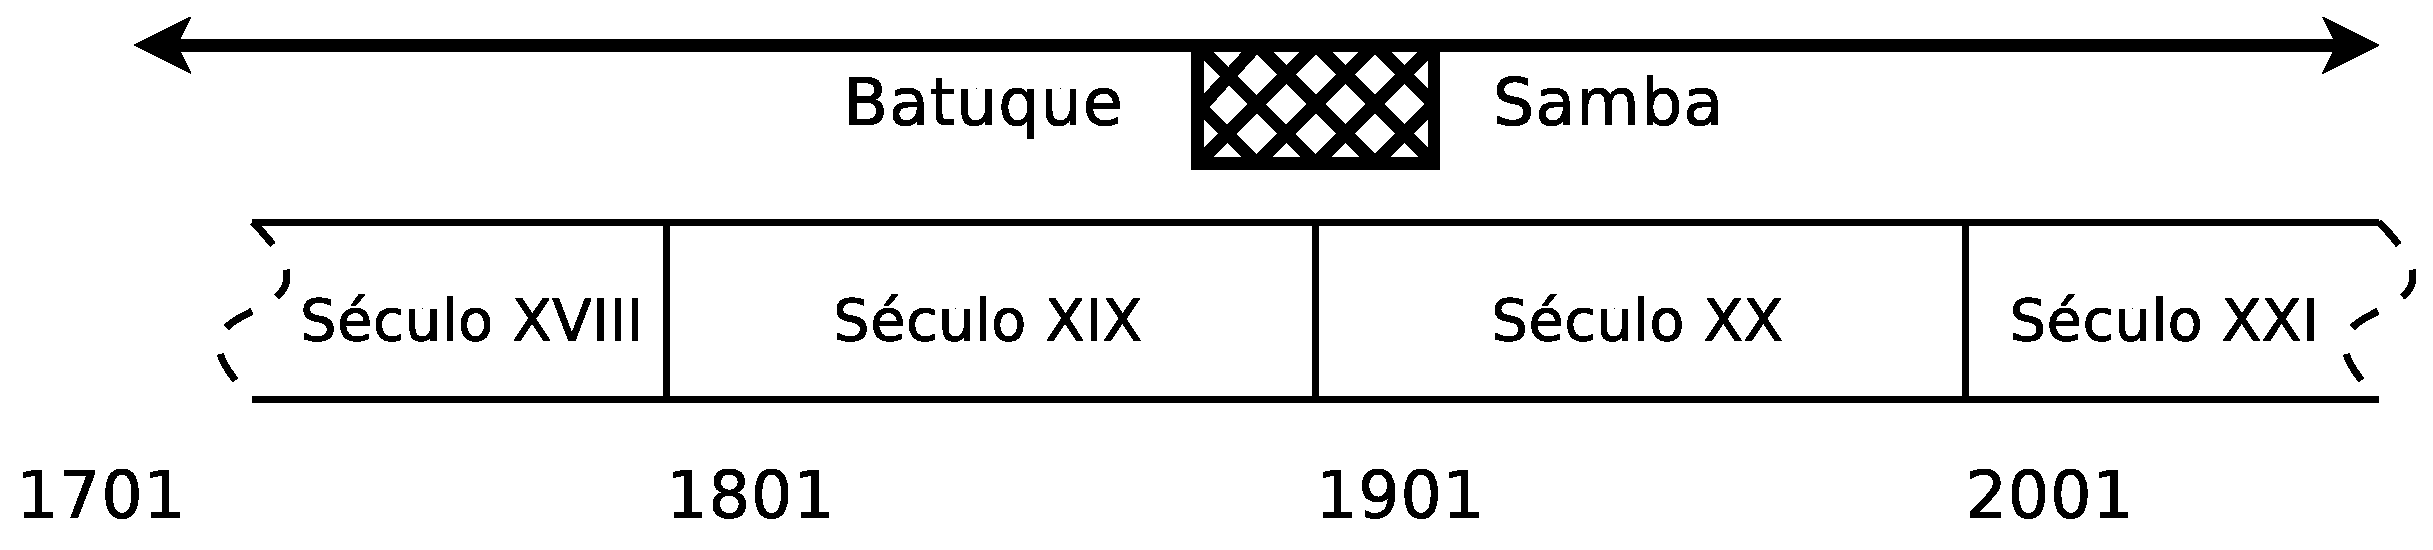
\includegraphics[width=0.85\textwidth]{chapters/cap-intro/samba-crono.eps}
  \caption{Cronologia da designação geral das danças Afro-brasileiras no Brasil.}
  \label{fig:sambacrono}
\end{figure}

Na literatura latino-americana a palavra ``samba'' é conhecida desde no seculo XIX, 
e na literatura brasileira desde o ano de 1838; porem, sendo a palavra ``samba''
quase desconhecida (em Rio de Janeiro) ate o último quartel do século XIX  \cite[pp. 47]{diniz2008almanaque}\cite[pp. 86]{sandroni2001feitico},
entre as explicações
do origem da palavra ``samba'' a mais conhecida é a que promove que esta vem 
do idioma quimbundo, sendo derivado da palavra ``semba''  que significa umbigada \cite[pp. 47]{diniz2008almanaque} \cite[pp. 50]{da2015historia}.
Uma referencia muito conhecida deste vinculo é a descrita no livro ``O negro e o garimpo em Minas Gerais''
de Mata Machado Filho, onde ele comenta que ``os negros corrigem para semba se 
alguém lhes fala em samba'' \cite[pp. 85]{sandroni2001feitico}. Assim se vê que existe
desde antanho uma relação entre as palavras, 
samba, semba e umbigada.


Entre as danças "profanas"\cite[pp. 85]{sandroni2001feitico} afro-brasileiras o gesto da umbigada é um elemento muito caraterístico,
de modo que em 1961 (seculo XX) Edson Carneiro definiu englobou as danças que realizam este 
gesto como ``samba-de-umbigada'' . Assim tradições 
musicais como o samba de roda, o jongo, o lundu, o coco, o calango e o cateretê, 
seguindo Edson são englobadas com  ``samba-de-umbigada'' \cite[pp. 85]{sandroni2001feitico}.



%%%%%%%%%%%%%%%%%%%%%%%%%%%%%%%%%%%%%%%%%%%%%%%%%%%%%%%%%%%%%%%%%%%%%%%%%%%%%%%%
%% SECTION
%%%%%%%%%%%%%%%%%%%%%%%%%%%%%%%%%%%%%%%%%%%%%%%%%%%%%%%%%%%%%%%%%%%%%%%%%%%%%%%%
\section{Historia das gafieiras}\index{historia das gafieiras}




Desde inícios do século XX já existiam associações para negros e mestiços, 
com distintas  finalidades, entre elas estava a criação de "sociedades dançantes ou recreativas", 
abertas a um publico geral
\cite[pp. 154-155]{neres1999negro} \cite[pp. 71]{de2008bexiga}.
Estas associações geralmente não tinham local próprio, 
e tinham que alugar espaços que terminavam sendo salões de velhos sobrados
ou similares \cite[pp. 154-155]{neres1999negro} \cite[pp. 49]{diniz2003almanaque}.
Por exemplo, no livro "O cabrocha" podemos ver uma descrição; escrita  por Jota Efegê em 1931; 
da "Sociedade Recreativa Familiar Bohemios de Botafogo" \cite{jotaefege},
a continuação é mostrado um extracto desse texto:

\begin{tcolorbox}[colback=lowgray,colframe=lowgray]%%
O salão, comquanto não fosse de grandes dimensões, era
de um tamanho regular, confinando com uma pequena saleta
onde tambem se dansava; estava bem affluido. Numa
heterogeneidade foliã, via-se desde a crioulinha blasée, sem
elegancia, desalinhada, á mulatinha pernostica de faces
avermelhadas por um carmin berrante, cabello engommado e
subjugado por travessas e grampos, num á la garçonne
forçado, mas exigido pela moda. Em meio dessas "cabrochas"
e "roxinhas", viam-se algumas moças brancas de apparencia
sobria. São as meninas que não podem fazer um vestido de
seda ou calçar sapatos de setim, para se apresentarem no
Fluminense ou no Flamengo e que nestes clubes se divertem,
ficando em evidencia por serem brancas.
~\\
(Jota Efegê)
\end{tcolorbox}



~\\
Apos a morte de um antigo socio na "Kananga do japao", Júlio simões decide fundar em 1930  
outro local de danças chamado "Elite clube" \cite[pp. 84]{cabral1996escolas} \cite[pp. 188]{raca1999},
na Rua Frei Caneca, 4 - Centro, Rio de Janeiro - RJ \cite{cabral2016elisete}.

\textcolor{red}{gafes \cite[pp. 188]{raca1999}.}


O termo gafieira foi criado pelo cronista carnavalesco, Romeu Arêde \cite[pp. 21]{efege1974maxixe} \cite[pp. 78]{coutinho2006cronistas}
(Em algumas versões é Romeu Aredo \cite[pp. 188]{raca1999}), 
também conhecido como "Picareta".
~\\


Devido a la denominação pejorativa de chamar a seu local um lugar de "gafes",
Júlio simões decide, em tom de zombaria, renomear seu local como "Gafieira Elite Clube" \cite[pp. 79]{moura1995tia},
sendo considerado por este fato a primeira gafieira do Brasil \cite{cabral2016elisete}.


Nesse ponto o nome "gafieira" cobrou relevância, e locais de dança conhecidos como gafieiras surgiram no Rio de Janeiro;
depois de tudo, já existissem lugares com estas caraterísticas desde inícios do século XX \cite[pp. 49]{diniz2003almanaque}, 
sendo estos lugares de esparzimento para os mestiços e negros da época.
Este salões foram criadas a semelhança dos bailes de salão da classe média ou alta \cite[pp. 78]{coutinho2006cronistas}; porem, no
caso das gafieiras, pela amplitude do seu públicos, tinham uma etiqueta cheia de equívocos (gaffes) \cite[pp. 49]{diniz2003almanaque},
ver Figura \ref{fig:gafieiracrono}.
\begin{figure}[h]
  \centering
    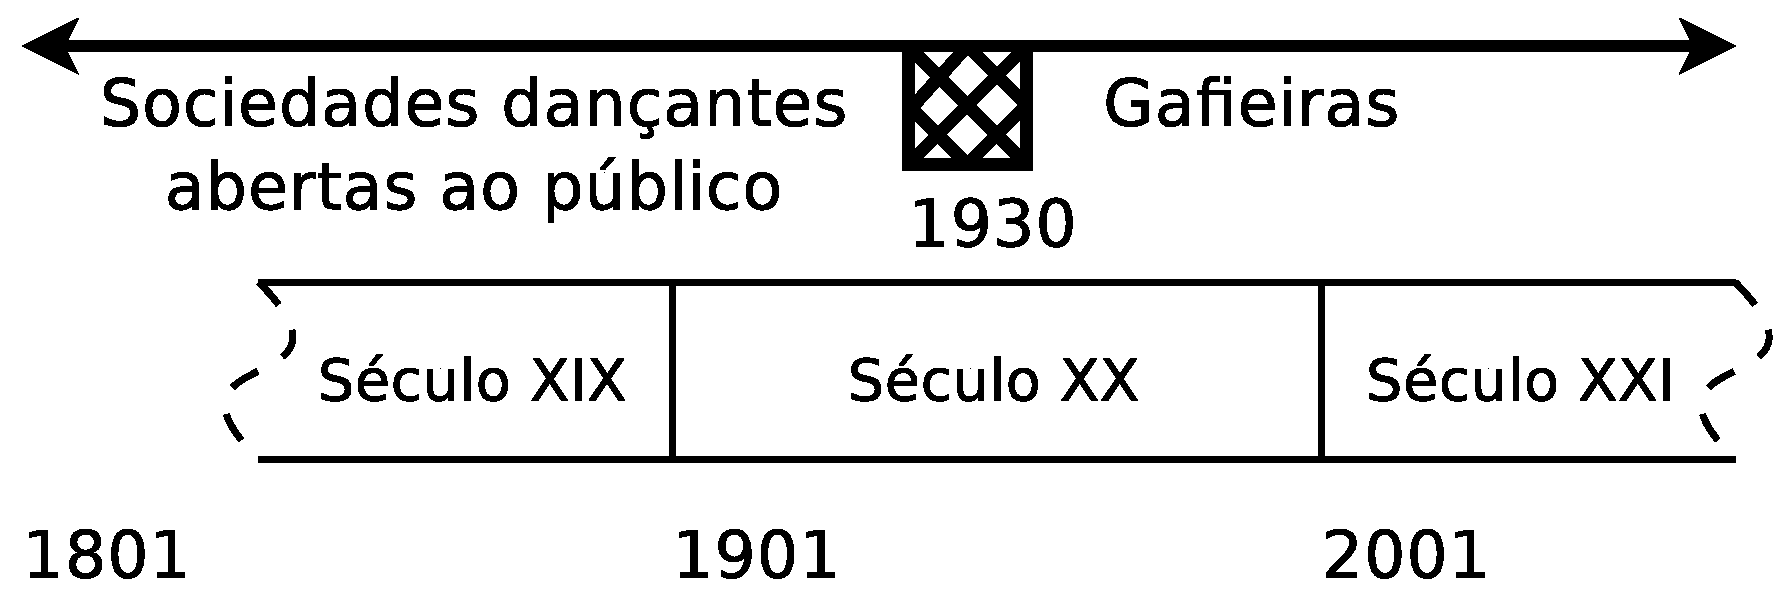
\includegraphics[width=0.65\textwidth]{chapters/cap-intro/gafieira-crono.eps}
  \caption{Cronologia da designação de gafieira para os salões de dança no Rio de janeiro.}
  \label{fig:gafieiracrono}
\end{figure}




%\newpage 
%%%%%%%%%%%%%%%%%%%%%%%%%%%%%%%%%%%%%%%%%%%%%%%%%%%%%%%%%%%%%%%%%%%%%%%%%%%%%%%%
%% SECTION
%%%%%%%%%%%%%%%%%%%%%%%%%%%%%%%%%%%%%%%%%%%%%%%%%%%%%%%%%%%%%%%%%%%%%%%%%%%%%%%%
\subsection{Estatutos da gafieira}\index{Estatuto da Gafieira}
Os "Estatutos da Gafieira" é uma composição musical escrita, por Billy Blanco;
esta foi interpretada por primeira vez na voz de Inezita Barroso, 
numa gravação da "RCA Victor" em janeiro de 1954 \cite{musicaestatuto};
O seguinte texto mostra a letra da música.
\begin{tcolorbox}[colback=lowgray,colframe=lowgray]%%
\center{Moço, olha o vexame,}\\
O ambiente exige respeito,\\
Pelos estatutos da nossa gafieira,\\
Dance a noite inteira, mas dance direito!\\
Aliás, pelo artigo 120,\\
O cavalheiro que fizer o seguinte:\\
Subir na parede, dançar de pé pro ar,\\
Morar na bebida sem querer pagar,\\
Abusar da umbigada de maneira folgazã,\\
Prejudicando hoje o bom crioulo de amanhã,\\
Será distintamente censurado,\\
Se balançar o corpo, vai pra mão do delegado.\\
Tá bem, moço?\\
\end{tcolorbox}
O texto é uma tentativa bem-humorada do autor de descrever o que acontecia 
nas gafieiras, porem na época da escrita desta popular samba, não
existiam tais regras, isto é confirmado por um depoimento realizado por 
Billy Blanco no 8 de julho de 2011 \cite{depoimentobilly}; o texto a seguir
mostra um fragmento dessa entrevista.

\begin{tcolorbox}[colback=lowgray,colframe=lowgray]%%
"Observando os acontecimentos de uma gafieira, então, eu imaginei
coisas, porque o compositor vive muito da imaginação. E eu criava situações 
possíveis de serem acontecidas na gafieira, ou então narrava o que
acontecia realmente. Por exemplo, no [samba] Pistom de Gafieira, tinha
um cidadão que era pistonista da orquestra que sempre tocava forte para
disfarçar quando a polícia vinha chegando. Doutra feita, eu tive a ideia
de fazer o estatuto para a gafieira. Então eu humorizei, porque ninguém
dança de pé pro ar, nem sobe em parede, não é? Mas a gente cria uma
extravagância dessas para dar uma certa graça, um certo sentido à música.
Na época, não havia código nenhum, eu apenas criei aquilo e muitas gafieiras 
depois tinham esse estatuto na parede para quem quisesse cantar.
Você vê que as regras do estatuto são umas regras brincalhonas, não é?" 
~\\
(Billy Blanco)
\end{tcolorbox}

Mesmo observando que as regras propostas pelo autor tem um caráter humorístico e sarcástico,
o texto foi adotado rapidamente pelas gafieiras, como um chamado a reflexão sobre umas
normas básicas a serem tidas em conta no salão. Por exemplo: 
A linha 7, pode ser interpretada como uma indicação a 
não fazer movimentos aéreos na pista de dança,
ou  evitar movimentos capoerísticos; tudo isto
pelo evidente espacio reduzido e compartilhado que existe na pista de dança, 
além de que os movimentos aéreos estão pensados para ser
executados em apresentações e não em danças sociais. 
A linha 8, nos lembra o respeito ao parceiro; pois a pessoa que dança precisa
estar no controle de suas faculdades físicas e mentais; 
no caso dos condutores\footnote{\label{footlab:conducao}Nas danças sociais é comunmente usado o paradigma 
da condução, onde no casal uma pessoa asume o papel de condutor dos movimentos e 
a outra pessoa, o seguidor, recebe a informação da condução e retorna uma resposta corporal.}, 
para estar atentos ao salão e cuidar do seu par enquanto os movimentos são executados, 
e no caso do seguidor\footref{footlab:conducao} para evitar problemas
nos giros e outros movimentos que precisem  controle do eixo do corpo.
As linhas 9 e 10 indicam sobre um conjunto de expressões artísticas 
afro-brasileiras emolduradas no século XIX com o nome de "samba umbigada",
posteriormente no mesmo seculo como "batuque" e finalmente no inícios do seculo XX foi chamado só 
de "samba" \cite[pp. 47]{diniz2008almanaque} \cite[pp. 85]{sandroni2001feitico}; nestas danças existe
um movimento chamado "umbigada" \cite{da2015historia} que da nome à dança, onde o ventre do homem e da mulher batem geralmente para indicar
a troca de dançarino; assim as linhas 9 e 10 se referem a
 evitar "abusar" de movimentos de umbigada que provem de danças que não eram bem vistas na época e eram consideradas gentílicas \cite[pp. 85]{sandroni2001feitico}.
Finalmente,
a linha 12 fala sobre balançar o corpo, que seguindo o contexto cultural, 
pode indicar não agir como bebado\cite{diccionario1858}, ou em outras palavras,
com pouca elegancia ou respeito,
caso contrario seria levado à delegacia!.


%\newpage 



%%%%%%%%%%%%%%%%%%%%%%%%%%%%%%%%%%%%%%%%%%%%%%%%%%%%%%%%%%%%%%%%%%%%%%%%%%%%%%%%
%% SECTION
%%%%%%%%%%%%%%%%%%%%%%%%%%%%%%%%%%%%%%%%%%%%%%%%%%%%%%%%%%%%%%%%%%%%%%%%%%%%%%%%
\section{Historia da samba de gafieira}\index{historia da samba de gafieira}


\textcolor{red}{Historia}
\begin{description}

\item [A] Perna, Marco Antonio (2001). Samba de Gafieira - a história da dança de salão brasileira. ISBN 85-901965-5-0

\end{description}




